\section{Analysis}
This chapter describes the first step of this project, the research of published technical reports and tools which are considered interesting for this project.
\subsection{BloodHound / SharpHound}
%Lukas
BloodHound describes itself on its wiki page on GitHub as follows:
\begin{quotation} \ \\
\textit{''BloodHound is a single page Javascript web application, built on top of Linkurious, compiled with Electron, with a Neo4j database fed by a PowerShell/C\# ingestor. \\
\ \\
BloodHound uses graph theory to reveal the hidden and often unintended relationships within an Active Directory environment. Attacks can use BloodHound to easily identify highly complex attack paths that would otherwise be impossible to quickly identify. Defenders can use BloodHound to identify and eliminate those same attack paths. Both blue and red teams can use BloodHound to easily gain a deeper understanding of privilege relationships in an Active Directory environment.''} 
\cite{blo2018}
\end{quotation}
\ \\
BloodHound was tested in the test environment describes later in this chapter. Both, the C\# and Python ingestors were successfully installed and tested. The only problem which occurred was that the Python-ingestor does not yet run on the latest Python release. One must have a Python 2.7.x version installed to run the scripts successfully.
The, for our project, most interesting part about BloodHound is the way they retrieve their data. \ \\
\ \\
Due to the decision that the application, in a first step, only reads the data of the local computer and not the whole domain, BloodHound will only be important in a later part of the project.

\subsection{WEFFLES}
%Lukas
WEFFLES (Windows Event Logging Forensic Logging Enhancement Services) is a Threat Hunting/Incident Response Console with Windows Event Forwarding and PowerBI, coded and published by Microsoft-Security-Employee Jessica Payne. It is build to help setting up the Windows Event Forwarding, so that all the collected logs of a system are stored on one centralized server, and afterwards to analyse the collected data. Jessica Payne wrote an installation instruction on the Microsoft TechNet blog \url{https://blogs.technet.microsoft.com/jepayne/2017/12/08/weffles/}. Once the data is collected on could simply import the generated weffels.csv file into Excel an start filtering the logs to gain the needed. Jessica Payne recommends to use PowerBI, a business analytics tool designed by Microsoft. In her published blog she also gives a short introduction on what to look out for, which event ids are important and other useful tips and tricks for detecting suspicious activities in the network.\ \\
\ \\
WEFFELS will not be the product on which this project is based, but could become an important point of reference. 
%Vilicht no persöliche ergänzig

\subsection{Microsoft Security Compliance Toolkit}
\subsubsection{Description}
The Microsoft Security Compliance Toolkit (SCT) \cite{SCT} allows security administrators to analyze their configured enterprise Group Policy Objects (GPO) in comparison to the Microsoft-recommended GPO baselines. The toolkit is handed with several baseline GPO's for different versions of Microsoft Windows Client and Servers:

\begin{itemize}
    \item Windows 10 security baselines
    \begin{itemize}
        \item Windows 10 Version 1803 (April 2018 Update)
        \item Windows 10 Version 1709 (Fall Creators Update)
        \item Windows 10 Version 1703 (Creators Update)
        \item Windows 10 Version 1607 (Anniversary Update)
        \item Windows 10 Version 1511 (November Update)
        \item Windows 10 Version 1507
    \end{itemize}
    \item Windows Server security baselines
    \begin{itemize}
        \item Windows Server 2016
        \item Windows Server 2012 R2
    \end{itemize}
    \item Microsoft Office security baseline
    \begin{itemize}
        \item Office 2016
    \end{itemize}
\end{itemize}

\subsubsection{Difficulties}
The toolkit is very simple and could be understood and used without any difficulties. The handling is very intuitive and does not require much training. Please note, however, that the toolkit cannot be used with Windows 10 Home, since active directory support is not provided with this version.

\subsubsection{Conclussion}
This toolkit can be used for a very baseline GPO in enterprise environment. With the handed baselines it is easy to compare the configured GPO and to see the readiness of the enterprise GPO. The toolkit gives also the ability to compare different local GPO's installed on different Clients or Servers to check their consistency. In addition the handed baselines can be used for building new GPO's.
\\\\
This toolkit is very interesting, but cannot be used to build on it. The reason for this is that the source code of the complete toolkit is not available. However, it can be used as additional help for checking the readiness of an enterprise environment.

\subsection{Microsoft Monitoring Active Directory for Signs of Compromise
}
\subsubsection{Description}
This article \cite{MSADSignsOfCompromise} is about configuration of an solid event log monitoring for Microsoft servers. The article gives a quiet well overview about the audit policy in Microsoft systems and what each policy stands for. The article gives information about the most important audit policies and how noisy (if a lot of data is produced by them) they are. This study does not go into the details of the audit policies in detail. Furthermore the article describes how the policies can be read with powershell.
\\\\
To this article Microsoft compiles in Appendix L \cite{MSAppendixL} all important event ids which are necessary for a successful detection of APTs and lateral movements.

\subsubsection{Conclussion}
Due to the fact that audit policies are an important setting for solid event logging, this article and appendix L will be a central part of the toolkit to be built. As a next step and part of this study these event ids have to be correlated with the event ids found in the JPCERT/CC's study "Detecting Lateral Movement through Tracking Event Logs" \cite{JPCERTDetectingLateralMovement} to make a clear statement which event ids have to be logged.

\subsection{MITRE ATT\&CK}
%Claudio

\subsection{JPCERT/CC - Detecting Lateral Movement through Tracking Event Logs}
%Lukas
This is a document the Japan Computer Emergency Response Team Coordination Center, or short JPCERT/CC, has published in the year 2017. It describes how, in their experience, attackers proceed with lateral movement. In a very detailed 81-page report they describe step by step the procedure, the tools used and what is most interesting for the project, the logs generated while doing so.
\\\\
This report is going to have a big impact on this project, it shows which logs have to be read in any case.

\subsection{JPCERT/CC - Detecting Lateral Movement in APTs} \label{DetectingLateral}
%Lukas
This document is from a presentation by Shingo Abe, a JPCERT/CC employee. In it he describes how to find system intruders more effectively using Windows Event Logs. The collected data is used to better detect inconsistencies, such as when an administrator logs on to another machine or when an administrator logs on suspiciously often. 
\\\\
This presentation contains interesting information which could be built into the project at a later point.

\subsection{LogonTracer}
\subsubsection{Description}
The LogonTracer is a tool built to investigate malicious logons on a system based on the research described in section \ref{DetectingLateral} \nameref{DetectingLateral}. The tool links hostnames or IP addresses with the \textit{"account name found in logon-related events and displays it as a graph"}. \cite{LogonTracer}

\subsubsection{Difficulties}

\subsubsection{Conclussion}


\subsection{Test environment}
A virtual network was set up on Azure-Cloud as a test environment. The test network was set up in the cloud so that the development team can access the network regardless of its location. The test network consists of a Windows server and two Windows clients. Active Directory service was configured on the server to manage the client computer. The following operating systems were installed in this test network: \\
\\
\textbf{Server:}
\begin{itemize}
    \item Windows Server 2016
\end{itemize}
\textbf{Clients:}
\begin{itemize}
    \item Windows 10 Pro, Version 1709
\end{itemize}
The network is structured as followed:\\
\begin{figure}[H]
    \centering
    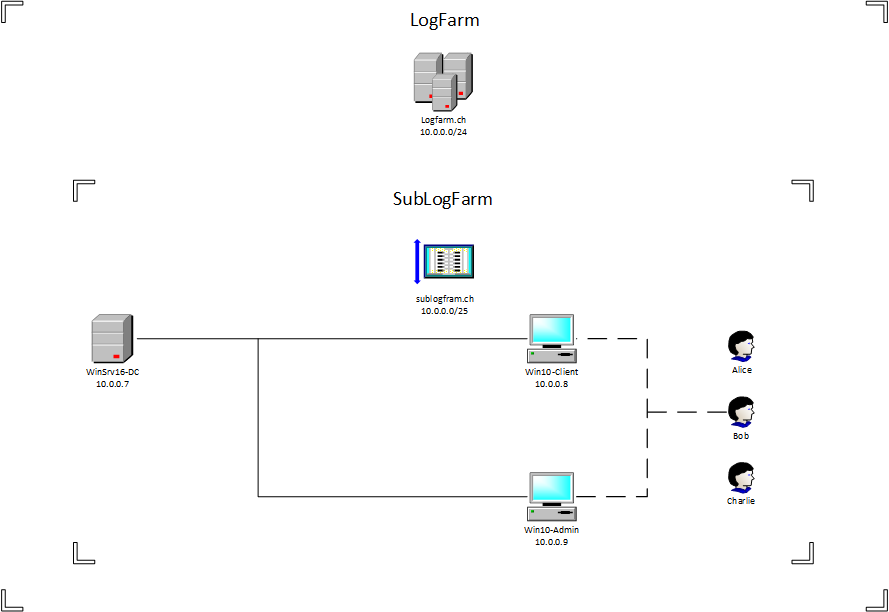
\includegraphics[width=0.9\linewidth]{assets/testnetwork.png}
    \caption{Test Environment}
\end{figure}
\subsubsection{Users}
Three different users were configured:
\begin{table}[H]
    \centering
    \begin{tabular}{p{4cm} p{8cm}} \hline
        \textbf{Name} & \textbf{Permissions}  \\ \hline
        alice & administrator  \\ \hline
        bob & user  \\ \hline
        charlie & user  \\ \hline
    \end{tabular}
    \caption{Test Environment Users}
\end{table}